\documentclass[tikz,border=6pt]{standalone}
\usetikzlibrary{calc}

% Gerado pelo MOIRA a partir do diagrama.
%
% Documento completo: compila direto com pdflatex.
%
% As posições são coordenadas nomeadas: mover um tensor é mudar uma linha
% da lista abaixo, e as pernas e as curvas o acompanham.

% Paleta da identidade MOIRA. Trocar a figura inteira de cor é mudar aqui.
\definecolor{moiraInk}{HTML}{1B2430}
\definecolor{moiraCyan}{HTML}{66CCEE}
\definecolor{moiraBlue}{HTML}{4477AA}
\definecolor{moiraAmber}{HTML}{CCBB44}
\definecolor{moiraGreen}{HTML}{228833}

\begin{document}
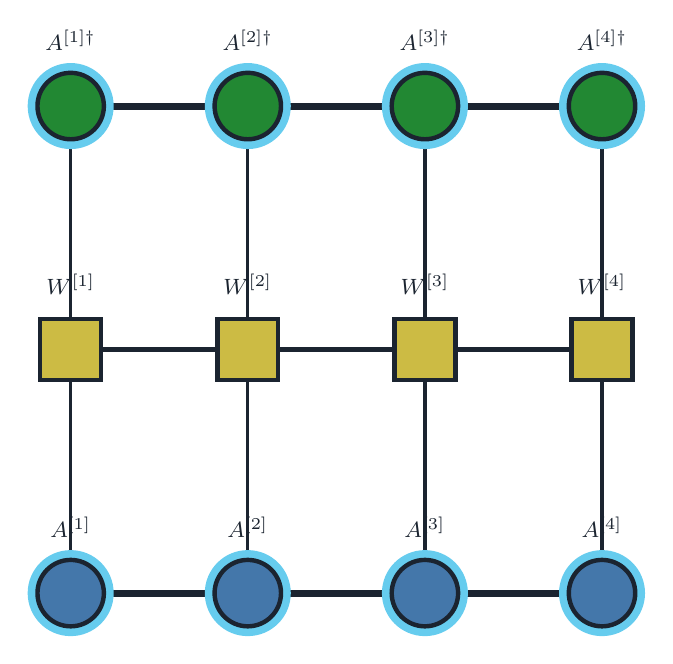
\begin{tikzpicture}[
    x=1pt, y=-1pt,
    moira bond/.style={draw=moiraInk, line cap=round},
    moira leg/.style={draw=moiraInk, line cap=round},
    moira shape/.style={draw=moiraInk, line width=1.6pt},
    moira ring/.style={line width=3pt},
    moira name/.style={text=moiraInk, font=\footnotesize, inner sep=1pt},
]

  % Posições dos tensores.
  \coordinate (t-t1) at (-96,88);
  \coordinate (t-t2) at (-32,88);
  \coordinate (t-t3) at (32,88);
  \coordinate (t-t4) at (96,88);
  \coordinate (t-t5) at (-96,0);
  \coordinate (t-t6) at (-32,0);
  \coordinate (t-t7) at (32,0);
  \coordinate (t-t8) at (96,0);
  \coordinate (t-t9) at (-96,-88);
  \coordinate (t-t10) at (-32,-88);
  \coordinate (t-t11) at (32,-88);
  \coordinate (t-t12) at (96,-88);

  % Vínculos.
  \draw[moira bond, line width=2.51pt] ($(t-t1)+(12,0)$) .. controls ($(t-t1)+(38,0)$) and ($(t-t2)+(-38,0)$) .. ($(t-t2)+(-12,0)$);
  \draw[moira bond, line width=2.51pt] ($(t-t2)+(12,0)$) .. controls ($(t-t2)+(38,0)$) and ($(t-t3)+(-38,0)$) .. ($(t-t3)+(-12,0)$);
  \draw[moira bond, line width=2.51pt] ($(t-t3)+(12,0)$) .. controls ($(t-t3)+(38,0)$) and ($(t-t4)+(-38,0)$) .. ($(t-t4)+(-12,0)$);
  \draw[moira bond, line width=2.07pt] ($(t-t5)+(11,0)$) .. controls ($(t-t5)+(37,0)$) and ($(t-t6)+(-37,0)$) .. ($(t-t6)+(-11,0)$);
  \draw[moira bond, line width=2.07pt] ($(t-t6)+(11,0)$) .. controls ($(t-t6)+(37,0)$) and ($(t-t7)+(-37,0)$) .. ($(t-t7)+(-11,0)$);
  \draw[moira bond, line width=2.07pt] ($(t-t7)+(11,0)$) .. controls ($(t-t7)+(37,0)$) and ($(t-t8)+(-37,0)$) .. ($(t-t8)+(-11,0)$);
  \draw[moira bond, line width=2.51pt] ($(t-t9)+(12,0)$) .. controls ($(t-t9)+(38,0)$) and ($(t-t10)+(-38,0)$) .. ($(t-t10)+(-12,0)$);
  \draw[moira bond, line width=2.51pt] ($(t-t10)+(12,0)$) .. controls ($(t-t10)+(38,0)$) and ($(t-t11)+(-38,0)$) .. ($(t-t11)+(-12,0)$);
  \draw[moira bond, line width=2.51pt] ($(t-t11)+(12,0)$) .. controls ($(t-t11)+(38,0)$) and ($(t-t12)+(-38,0)$) .. ($(t-t12)+(-12,0)$);
  \draw[moira bond, line width=1.2pt] ($(t-t1)+(0,-12)$) .. controls ($(t-t1)+(0,-38)$) and ($(t-t5)+(0,37)$) .. ($(t-t5)+(0,11)$);
  \draw[moira bond, line width=1.2pt] ($(t-t5)+(0,-11)$) .. controls ($(t-t5)+(0,-37)$) and ($(t-t9)+(0,38)$) .. ($(t-t9)+(0,12)$);
  \draw[moira bond, line width=1.2pt] ($(t-t2)+(0,-12)$) .. controls ($(t-t2)+(0,-38)$) and ($(t-t6)+(0,37)$) .. ($(t-t6)+(0,11)$);
  \draw[moira bond, line width=1.2pt] ($(t-t6)+(0,-11)$) .. controls ($(t-t6)+(0,-37)$) and ($(t-t10)+(0,38)$) .. ($(t-t10)+(0,12)$);
  \draw[moira bond, line width=1.2pt] ($(t-t3)+(0,-12)$) .. controls ($(t-t3)+(0,-38)$) and ($(t-t7)+(0,37)$) .. ($(t-t7)+(0,11)$);
  \draw[moira bond, line width=1.2pt] ($(t-t7)+(0,-11)$) .. controls ($(t-t7)+(0,-37)$) and ($(t-t11)+(0,38)$) .. ($(t-t11)+(0,12)$);
  \draw[moira bond, line width=1.2pt] ($(t-t4)+(0,-12)$) .. controls ($(t-t4)+(0,-38)$) and ($(t-t8)+(0,37)$) .. ($(t-t8)+(0,11)$);
  \draw[moira bond, line width=1.2pt] ($(t-t8)+(0,-11)$) .. controls ($(t-t8)+(0,-37)$) and ($(t-t12)+(0,38)$) .. ($(t-t12)+(0,12)$);

  % Tensores.
  \draw[moira ring, draw=moiraCyan] (t-t1) circle[radius=14.04pt];
  \draw[moira shape, fill=moiraBlue] (t-t1) circle[radius=12pt];
  \draw[moira ring, draw=moiraCyan] (t-t2) circle[radius=14.04pt];
  \draw[moira shape, fill=moiraBlue] (t-t2) circle[radius=12pt];
  \draw[moira ring, draw=moiraCyan] (t-t3) circle[radius=14.04pt];
  \draw[moira shape, fill=moiraBlue] (t-t3) circle[radius=12pt];
  \draw[moira ring, draw=moiraCyan] (t-t4) circle[radius=14.04pt];
  \draw[moira shape, fill=moiraBlue] (t-t4) circle[radius=12pt];
  \draw[moira shape, fill=moiraAmber] ($(t-t5)+(-11,-11)$) -- ($(t-t5)+(11,-11)$) -- ($(t-t5)+(11,11)$) -- ($(t-t5)+(-11,11)$) -- cycle;
  \draw[moira shape, fill=moiraAmber] ($(t-t6)+(-11,-11)$) -- ($(t-t6)+(11,-11)$) -- ($(t-t6)+(11,11)$) -- ($(t-t6)+(-11,11)$) -- cycle;
  \draw[moira shape, fill=moiraAmber] ($(t-t7)+(-11,-11)$) -- ($(t-t7)+(11,-11)$) -- ($(t-t7)+(11,11)$) -- ($(t-t7)+(-11,11)$) -- cycle;
  \draw[moira shape, fill=moiraAmber] ($(t-t8)+(-11,-11)$) -- ($(t-t8)+(11,-11)$) -- ($(t-t8)+(11,11)$) -- ($(t-t8)+(-11,11)$) -- cycle;
  \draw[moira ring, draw=moiraCyan] (t-t9) circle[radius=14.04pt];
  \draw[moira shape, fill=moiraGreen] (t-t9) circle[radius=12pt];
  \draw[moira ring, draw=moiraCyan] (t-t10) circle[radius=14.04pt];
  \draw[moira shape, fill=moiraGreen] (t-t10) circle[radius=12pt];
  \draw[moira ring, draw=moiraCyan] (t-t11) circle[radius=14.04pt];
  \draw[moira shape, fill=moiraGreen] (t-t11) circle[radius=12pt];
  \draw[moira ring, draw=moiraCyan] (t-t12) circle[radius=14.04pt];
  \draw[moira shape, fill=moiraGreen] (t-t12) circle[radius=12pt];

  % Rótulos.
  \node[moira name, anchor=base] at ($(t-t1)+(0,-20)$) {$A^{[1]}$};
  \node[moira name, anchor=base] at ($(t-t2)+(0,-20)$) {$A^{[2]}$};
  \node[moira name, anchor=base] at ($(t-t3)+(0,-20)$) {$A^{[3]}$};
  \node[moira name, anchor=base] at ($(t-t4)+(0,-20)$) {$A^{[4]}$};
  \node[moira name, anchor=base] at ($(t-t5)+(0,-20)$) {$W^{[1]}$};
  \node[moira name, anchor=base] at ($(t-t6)+(0,-20)$) {$W^{[2]}$};
  \node[moira name, anchor=base] at ($(t-t7)+(0,-20)$) {$W^{[3]}$};
  \node[moira name, anchor=base] at ($(t-t8)+(0,-20)$) {$W^{[4]}$};
  \node[moira name, anchor=base] at ($(t-t9)+(0,-20)$) {$A^{[1]\dagger}$};
  \node[moira name, anchor=base] at ($(t-t10)+(0,-20)$) {$A^{[2]\dagger}$};
  \node[moira name, anchor=base] at ($(t-t11)+(0,-20)$) {$A^{[3]\dagger}$};
  \node[moira name, anchor=base] at ($(t-t12)+(0,-20)$) {$A^{[4]\dagger}$};
\end{tikzpicture}
\end{document}
